\documentclass[letterpaper,12pt]{article}\usepackage[]{graphicx}\usepackage[]{color}
%% maxwidth is the original width if it is less than linewidth
%% otherwise use linewidth (to make sure the graphics do not exceed the margin)
\makeatletter
\def\maxwidth{ %
  \ifdim\Gin@nat@width>\linewidth
    \linewidth
  \else
    \Gin@nat@width
  \fi
}
\makeatother

\definecolor{fgcolor}{rgb}{0.345, 0.345, 0.345}
\newcommand{\hlnum}[1]{\textcolor[rgb]{0.686,0.059,0.569}{#1}}%
\newcommand{\hlstr}[1]{\textcolor[rgb]{0.192,0.494,0.8}{#1}}%
\newcommand{\hlcom}[1]{\textcolor[rgb]{0.678,0.584,0.686}{\textit{#1}}}%
\newcommand{\hlopt}[1]{\textcolor[rgb]{0,0,0}{#1}}%
\newcommand{\hlstd}[1]{\textcolor[rgb]{0.345,0.345,0.345}{#1}}%
\newcommand{\hlkwa}[1]{\textcolor[rgb]{0.161,0.373,0.58}{\textbf{#1}}}%
\newcommand{\hlkwb}[1]{\textcolor[rgb]{0.69,0.353,0.396}{#1}}%
\newcommand{\hlkwc}[1]{\textcolor[rgb]{0.333,0.667,0.333}{#1}}%
\newcommand{\hlkwd}[1]{\textcolor[rgb]{0.737,0.353,0.396}{\textbf{#1}}}%
\let\hlipl\hlkwb

\usepackage{framed}
\makeatletter
\newenvironment{kframe}{%
 \def\at@end@of@kframe{}%
 \ifinner\ifhmode%
  \def\at@end@of@kframe{\end{minipage}}%
  \begin{minipage}{\columnwidth}%
 \fi\fi%
 \def\FrameCommand##1{\hskip\@totalleftmargin \hskip-\fboxsep
 \colorbox{shadecolor}{##1}\hskip-\fboxsep
     % There is no \\@totalrightmargin, so:
     \hskip-\linewidth \hskip-\@totalleftmargin \hskip\columnwidth}%
 \MakeFramed {\advance\hsize-\width
   \@totalleftmargin\z@ \linewidth\hsize
   \@setminipage}}%
 {\par\unskip\endMakeFramed%
 \at@end@of@kframe}
\makeatother

\definecolor{shadecolor}{rgb}{.97, .97, .97}
\definecolor{messagecolor}{rgb}{0, 0, 0}
\definecolor{warningcolor}{rgb}{1, 0, 1}
\definecolor{errorcolor}{rgb}{1, 0, 0}
\newenvironment{knitrout}{}{} % an empty environment to be redefined in TeX

\usepackage{alltt}
\usepackage[top=1in,bottom=1in,left=1in,right=1in]{geometry}
\usepackage{setspace}
\usepackage[colorlinks=true,urlcolor=blue,citecolor=blue,linkcolor=blue]{hyperref}
\usepackage{indentfirst}
\usepackage{multirow}
\usepackage{booktabs}
\usepackage[final]{animate}
\usepackage{graphicx}
\usepackage{verbatim}
\usepackage{rotating}
\usepackage{tabularx}
\usepackage{array}
\usepackage{subfig} 
\usepackage[noae]{Sweave}
\usepackage{cleveref}
\usepackage[figureposition=bottom]{caption}
\usepackage{paralist}
\usepackage{acronym}
\usepackage{outlines}
\usepackage{pdflscape}

% housekeeping
\begin{knitrout}
\definecolor{shadecolor}{rgb}{0.969, 0.969, 0.969}\color{fgcolor}\begin{kframe}


{\ttfamily\noindent\color{warningcolor}{\#\# Warning: package 'tidyr' was built under R version 3.4.2}}

{\ttfamily\noindent\color{warningcolor}{\#\# Warning: package 'purrr' was built under R version 3.4.2}}

{\ttfamily\noindent\color{warningcolor}{\#\# Warning: package 'dplyr' was built under R version 3.4.2}}

{\ttfamily\noindent\color{warningcolor}{\#\# Warning: package 'GGally' was built under R version 3.4.2}}

{\ttfamily\noindent\color{warningcolor}{\#\# Warning: package 'glmulti' was built under R version 3.4.2}}

{\ttfamily\noindent\color{warningcolor}{\#\# Warning: package 'rJava' was built under R version 3.4.2}}

{\ttfamily\noindent\color{warningcolor}{\#\# Warning: package 'MuMIn' was built under R version 3.4.2}}\end{kframe}
\end{knitrout}

\linespread{1}
\IfFileExists{upquote.sty}{\usepackage{upquote}}{}
\begin{document}
\title{Analysis of crab abundance, presence/absence, and carapace length}
\maketitle



\begin{knitrout}
\definecolor{shadecolor}{rgb}{0.969, 0.969, 0.969}\color{fgcolor}
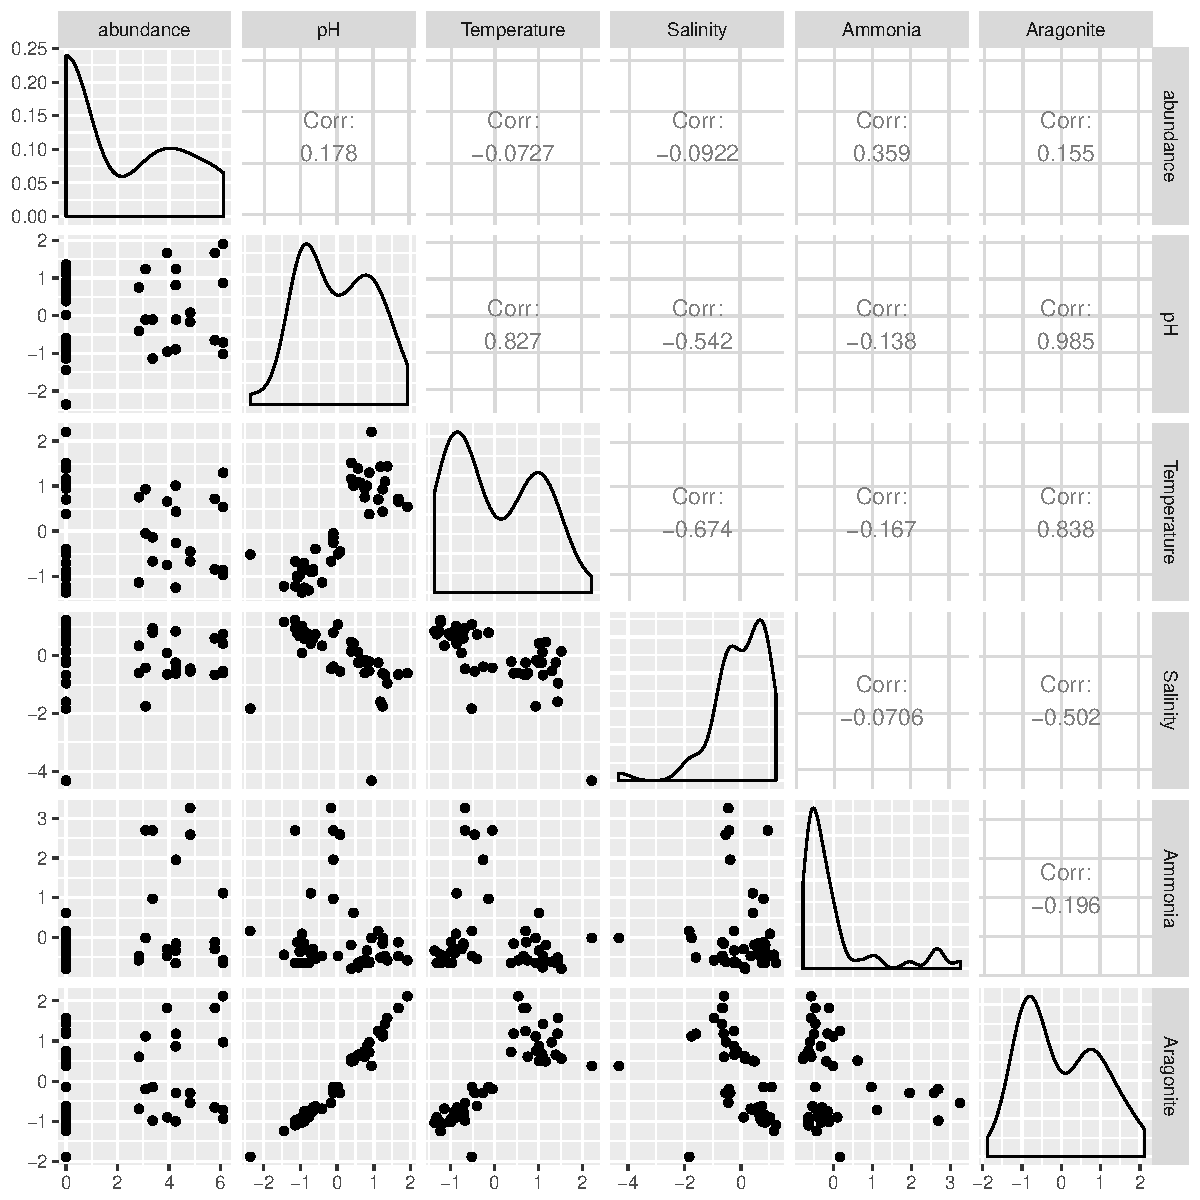
\includegraphics[width=\maxwidth]{figure/unnamed-chunk-3-1} 

\end{knitrout}



\begin{knitrout}
\definecolor{shadecolor}{rgb}{0.969, 0.969, 0.969}\color{fgcolor}\begin{figure}
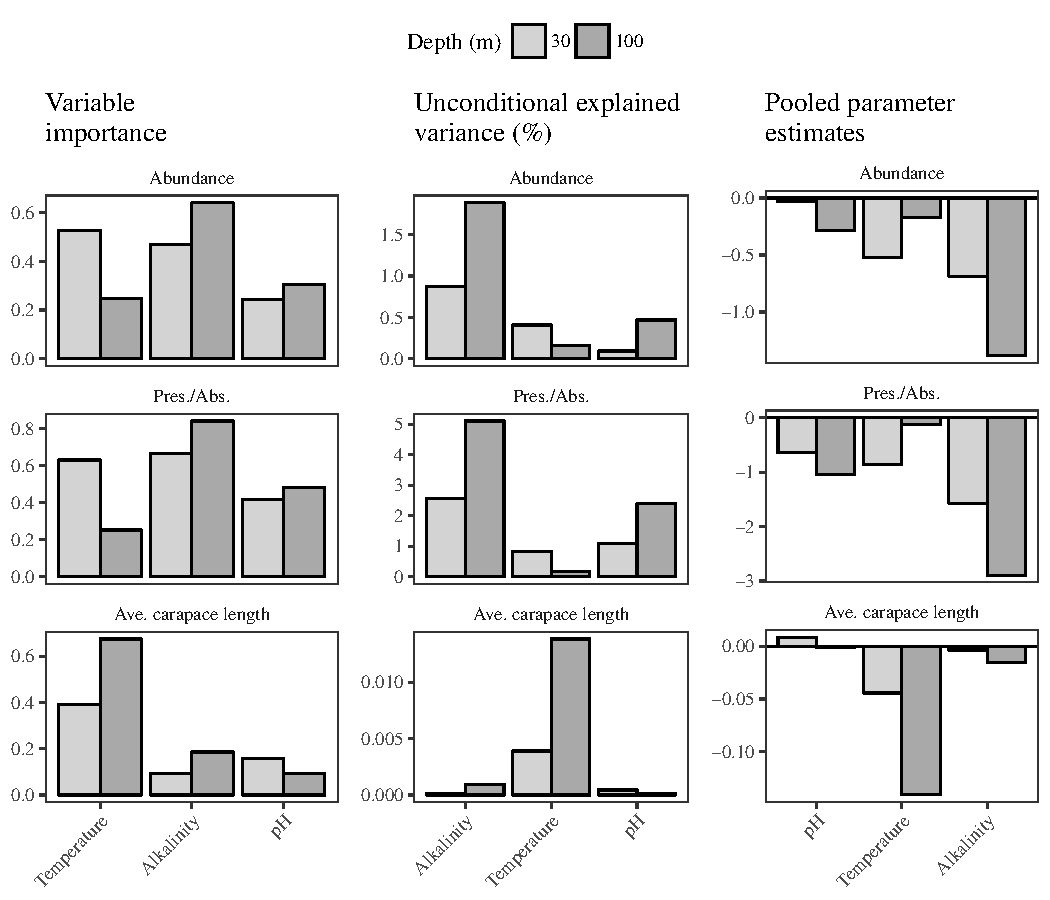
\includegraphics[width=\maxwidth]{figure/unnamed-chunk-5-1} \caption[Results of model selection analysis with three crab population variables (abundance, presence/absence, carapace length) by shallow and deep depths]{Results of model selection analysis with three crab population variables (abundance, presence/absence, carapace length) by shallow and deep depths. Variable importances and pooled estimates show summarized results from multiple models that evaluated all parameter combinations.  The unconditional explained variance (\%) is the effect of each variable independent of all other variables.}\label{fig:unnamed-chunk-5}
\end{figure}


\end{knitrout}
\clearpage

%latex.default(abutab[, -c(1, 2)], file = "", rowlabel = "Models",     caption = cap.val, caption.loc = "top", rgroup = names(table(abutab$depth)),     n.rgroup = table(abutab$depth), rowname = abutab$model, size = "footnotesize",     label = "tab:abutab")%
\begin{table}[!tbp]
{\footnotesize
\caption{Top five selected models for crab abundance at shallow and deep depths. Input variables were ammonia, aragonite, ph, salinity, and temperature. All explanatory variables were scaled and centered.\label{tab:abutab}} 
\begin{center}
\begin{tabular}{llllllllll}
\hline\hline
\multicolumn{1}{l}{Models}&\multicolumn{1}{c}{Int.}&\multicolumn{1}{c}{Ammonia}&\multicolumn{1}{c}{Aragonite}&\multicolumn{1}{c}{pH}&\multicolumn{1}{c}{Temperature}&\multicolumn{1}{c}{df}&\multicolumn{1}{c}{logLik}&\multicolumn{1}{c}{AICc}&\multicolumn{1}{c}{delta}\tabularnewline
\hline
{\bfseries 10 m}&&&&&&&&&\tabularnewline
~~1&1.63&-&-&2.15&-1.88&4&-49.42&108.95&0\tabularnewline
~~2&1.08&1.02&-&2.51&-1.37&5&-48.13&109.58&0.64\tabularnewline
~~3&0.41&1.72&2.08&-&-&4&-49.81&109.72&0.78\tabularnewline
~~4&0.17&1.55&-&2.32&-&4&-49.89&109.89&0.94\tabularnewline
~~5&1.31&1.22&2.18&-&-1.27&5&-48.29&109.9&0.96\tabularnewline
\hline
{\bfseries 200 m}&&&&&&&&&\tabularnewline
~~1&1.68&0.87&-&-&&3&-51.73&110.66&0\tabularnewline
~~2&4.35&-&2.89&-&&3&-52.22&111.65&0.99\tabularnewline
~~3&3.59&-&-&2.01&&3&-52.24&111.67&1.01\tabularnewline
~~4&2.87&0.66&-&1.33&&4&-50.87&111.84&1.18\tabularnewline
~~5&3.32&0.65&1.84&-&&4&-50.95&112&1.34\tabularnewline
\hline
\end{tabular}\end{center}}
\end{table}
%latex.default(patab[, -c(1, 2)], file = "", rowlabel = "Models",     caption = cap.val, caption.loc = "top", rgroup = names(table(patab$depth)),     n.rgroup = table(patab$depth), rowname = patab$model, size = "footnotesize",     label = "tab:patab")%
\begin{table}[!tbp]
{\footnotesize
\caption{Top five selected models for crab presence/absence at shallow and deep depths. Input variables were ammonia, aragonite, ph, salinity, and temperature. All explanatory variables were scaled and centered.\label{tab:patab}} 
\begin{center}
\begin{tabular}{lllllllllll}
\hline\hline
\multicolumn{1}{l}{Models}&\multicolumn{1}{c}{Int.}&\multicolumn{1}{c}{Ammonia}&\multicolumn{1}{c}{Aragonite}&\multicolumn{1}{c}{pH}&\multicolumn{1}{c}{Salinity}&\multicolumn{1}{c}{Temperature}&\multicolumn{1}{c}{df}&\multicolumn{1}{c}{logLik}&\multicolumn{1}{c}{AICc}&\multicolumn{1}{c}{delta}\tabularnewline
\hline
{\bfseries 10}&&&&&&&&&&\tabularnewline
~~1&-0.34&-&-&2.15&-&-2.32&3&-12.07&31.34&0\tabularnewline
~~2&0.07&-&1.73&-&-&-2.4&3&-12.41&32.01&0.68\tabularnewline
~~3&-0.83&1.48&-&2.63&-&-1.83&4&-10.99&32.09&0.75\tabularnewline
~~4&-1.87&1.93&-&2.12&-&-&3&-12.69&32.57&1.23\tabularnewline
~~5&1.41&-&-&-&-1.04&-2.7&3&-12.76&32.72&1.39\tabularnewline
\hline
{\bfseries 200}&&&&&&&&&&\tabularnewline
~~1&2.53&1.35&-&3.37&-&&3&-10.74&28.67&0\tabularnewline
~~2&-0.43&1.39&-&-&-&&2&-12.4&29.36&0.69\tabularnewline
~~3&2.85&1.19&3.77&-&-&&3&-11.18&29.57&0.9\tabularnewline
~~4&4.43&1.42&-&4.16&-1.86&&4&-9.94&29.98&1.31\tabularnewline
~~5&2.55&-&-&3.54&-&&2&-12.91&30.4&1.72\tabularnewline
\hline
\end{tabular}\end{center}}
\end{table}
%latex.default(cltab[, -c(1, 2)], file = "", rowlabel = "Models",     caption = cap.val, caption.loc = "top", rgroup = names(table(cltab$depth)),     n.rgroup = table(cltab$depth), rowname = cltab$model, size = "footnotesize",     label = "tab:cltab")%
\begin{table}[!tbp]
{\footnotesize
\caption{Top five selected models for crab carapace length at shallow and deep depths. Input variables were ammonia, aragonite, ph, salinity, and temperature.  All explanatory variables were scaled and centered.\label{tab:cltab}} 
\begin{center}
\begin{tabular}{lllllllllll}
\hline\hline
\multicolumn{1}{l}{Models}&\multicolumn{1}{c}{Int.}&\multicolumn{1}{c}{Ammonia}&\multicolumn{1}{c}{Aragonite}&\multicolumn{1}{c}{Salinity}&\multicolumn{1}{c}{Temperature}&\multicolumn{1}{c}{df}&\multicolumn{1}{c}{logLik}&\multicolumn{1}{c}{AICc}&\multicolumn{1}{c}{delta}&\multicolumn{1}{c}{pH}\tabularnewline
\hline
{\bfseries 10}&&&&&&&&&&\tabularnewline
~~1&6.59&-&-&-&-&2&6.99&-8.28&0&\tabularnewline
~~2&6.65&-&-&-&-0.11&3&8.27&-6.54&1.74&\tabularnewline
~~3&6.58&0.04&-&-&-&3&7.48&-4.97&3.31&\tabularnewline
~~4&6.62&-&-&0.06&-&3&7.43&-4.87&3.41&\tabularnewline
~~5&6.6&-&-0.01&-&-&3&7.02&-4.03&4.24&\tabularnewline
\hline
{\bfseries 200}&&&&&&&&&&\tabularnewline
~~1&6.59&&-&-&-&2&6.99&-8.28&0&-\tabularnewline
~~2&6.6&&-&-0.04&-&3&7.13&-4.26&4.02&-\tabularnewline
~~3&6.55&&-&-&-0.05&3&7.11&-4.23&4.05&-\tabularnewline
~~4&6.56&&-0.04&-&-&3&7.04&-4.08&4.2&-\tabularnewline
~~5&6.6&&-&-&-&3&7.03&-4.06&4.21&0.03\tabularnewline
\hline
\end{tabular}\end{center}}
\end{table}


\end{document}
